\section{Timed functions: \textit{libinger}}
\label{sec:libinger}

An application wishing to use preemptible functions links against our shared library,
\textit{libinger}\footnote{In the style of GNU's \textit{libiberty}, we named our
system for the command-line switch used to link against it.  As the proverb goes,
``Don't want your function calls to linger?  Link with \texttt{-linger}.''}, which
provides an API for making timed function calls.  This comprises two main functions
(Listing~\ref{lst:ingerapi}):
\begin{itemize}
\item \texttt{launch()} invokes an ordinary function $\mathcal{F}$ with an
execution time cap of $T$.  The call to \texttt{launch()} returns when $\mathcal{F}$
completes, or after approximately $T$ microseconds if $\mathcal{F}$ has not returned
by then.  In the latter case, \textit{libinger} returns an opaque continuation
object recording the intermediate execution state.
\item \texttt{resume()} may be called on the continuation generated by a single call
to \texttt{launch()} followed by zero or more calls to \texttt{resume()}.  If the
corresponding $\mathcal{F}$ had not yet returned, \textit{libinger} continues
executing it from the point last reached.
\end{itemize}

\begin{figure}
\begin{lstlisting}[label=lst:ingerapi,caption=Preemptible functions interface]
struct linger_t {
  bool is_complete;
  cont_t continuation;
};

linger_t launch(Function func,
                u64 time_us,
                void *args);
void resume(linger_t *cont, u64 time_us);
\end{lstlisting}
\end{figure}

Listing~\ref{lst:usage} shows an example usage of \textit{libinger}
in a task queue manager designed to prevent latency-critical tasks from blocking
behind longer-running
ones. The caller invokes a task with a timeout. If the task does not complete
within the allotted time, the caller saves its continuation in the task queue,
proceeds to handling other tasks, and later resumes the first task.

\begin{figure}
\begin{lstlisting}[label=lst:usage, caption=Preemptible function usage example]

linger = launch(task, TIMEOUT, null);
if (!linger.is_complete) {
  // Save @linger to a task queue to
  // resume later
  task_queue.push(linger);
}

// Handle other tasks
...
// Resume @task at some later point
linger = task_queue.pop();
resume(&linger, TIMEOUT);
\end{lstlisting}
\end{figure}

In accordance with our goal of language agnosticism, \textit{libinger} exposes both C
and Rust~\cite{www-rustlang} APIs.  To demonstrate the flexibility and composability
of the preemptible function abstraction, we have also created \textit{libturquoise},
a preemptive userland thread library, by porting an existing futures-based thread
pool to \textit{libinger}.  We discuss this system in Section~\ref{sec:libturquoise}.

Figure~\ref{fig:architecture} shows a dependency graph of the software components
comprising the preemptible functions stack.  The \textit{libinger} library itself is
implemented in approximately 2,500 lines of Rust.  To support calls to nonreentrant
functions, it depends on another library, \textit{libgotcha}, which consists of
another 3,000 lines of C, Rust, and x86-64 assembly.  We now describe the
implementation of \textit{libinger}, beginning with this shared state handling.

\begin{figure}
\begin{center}
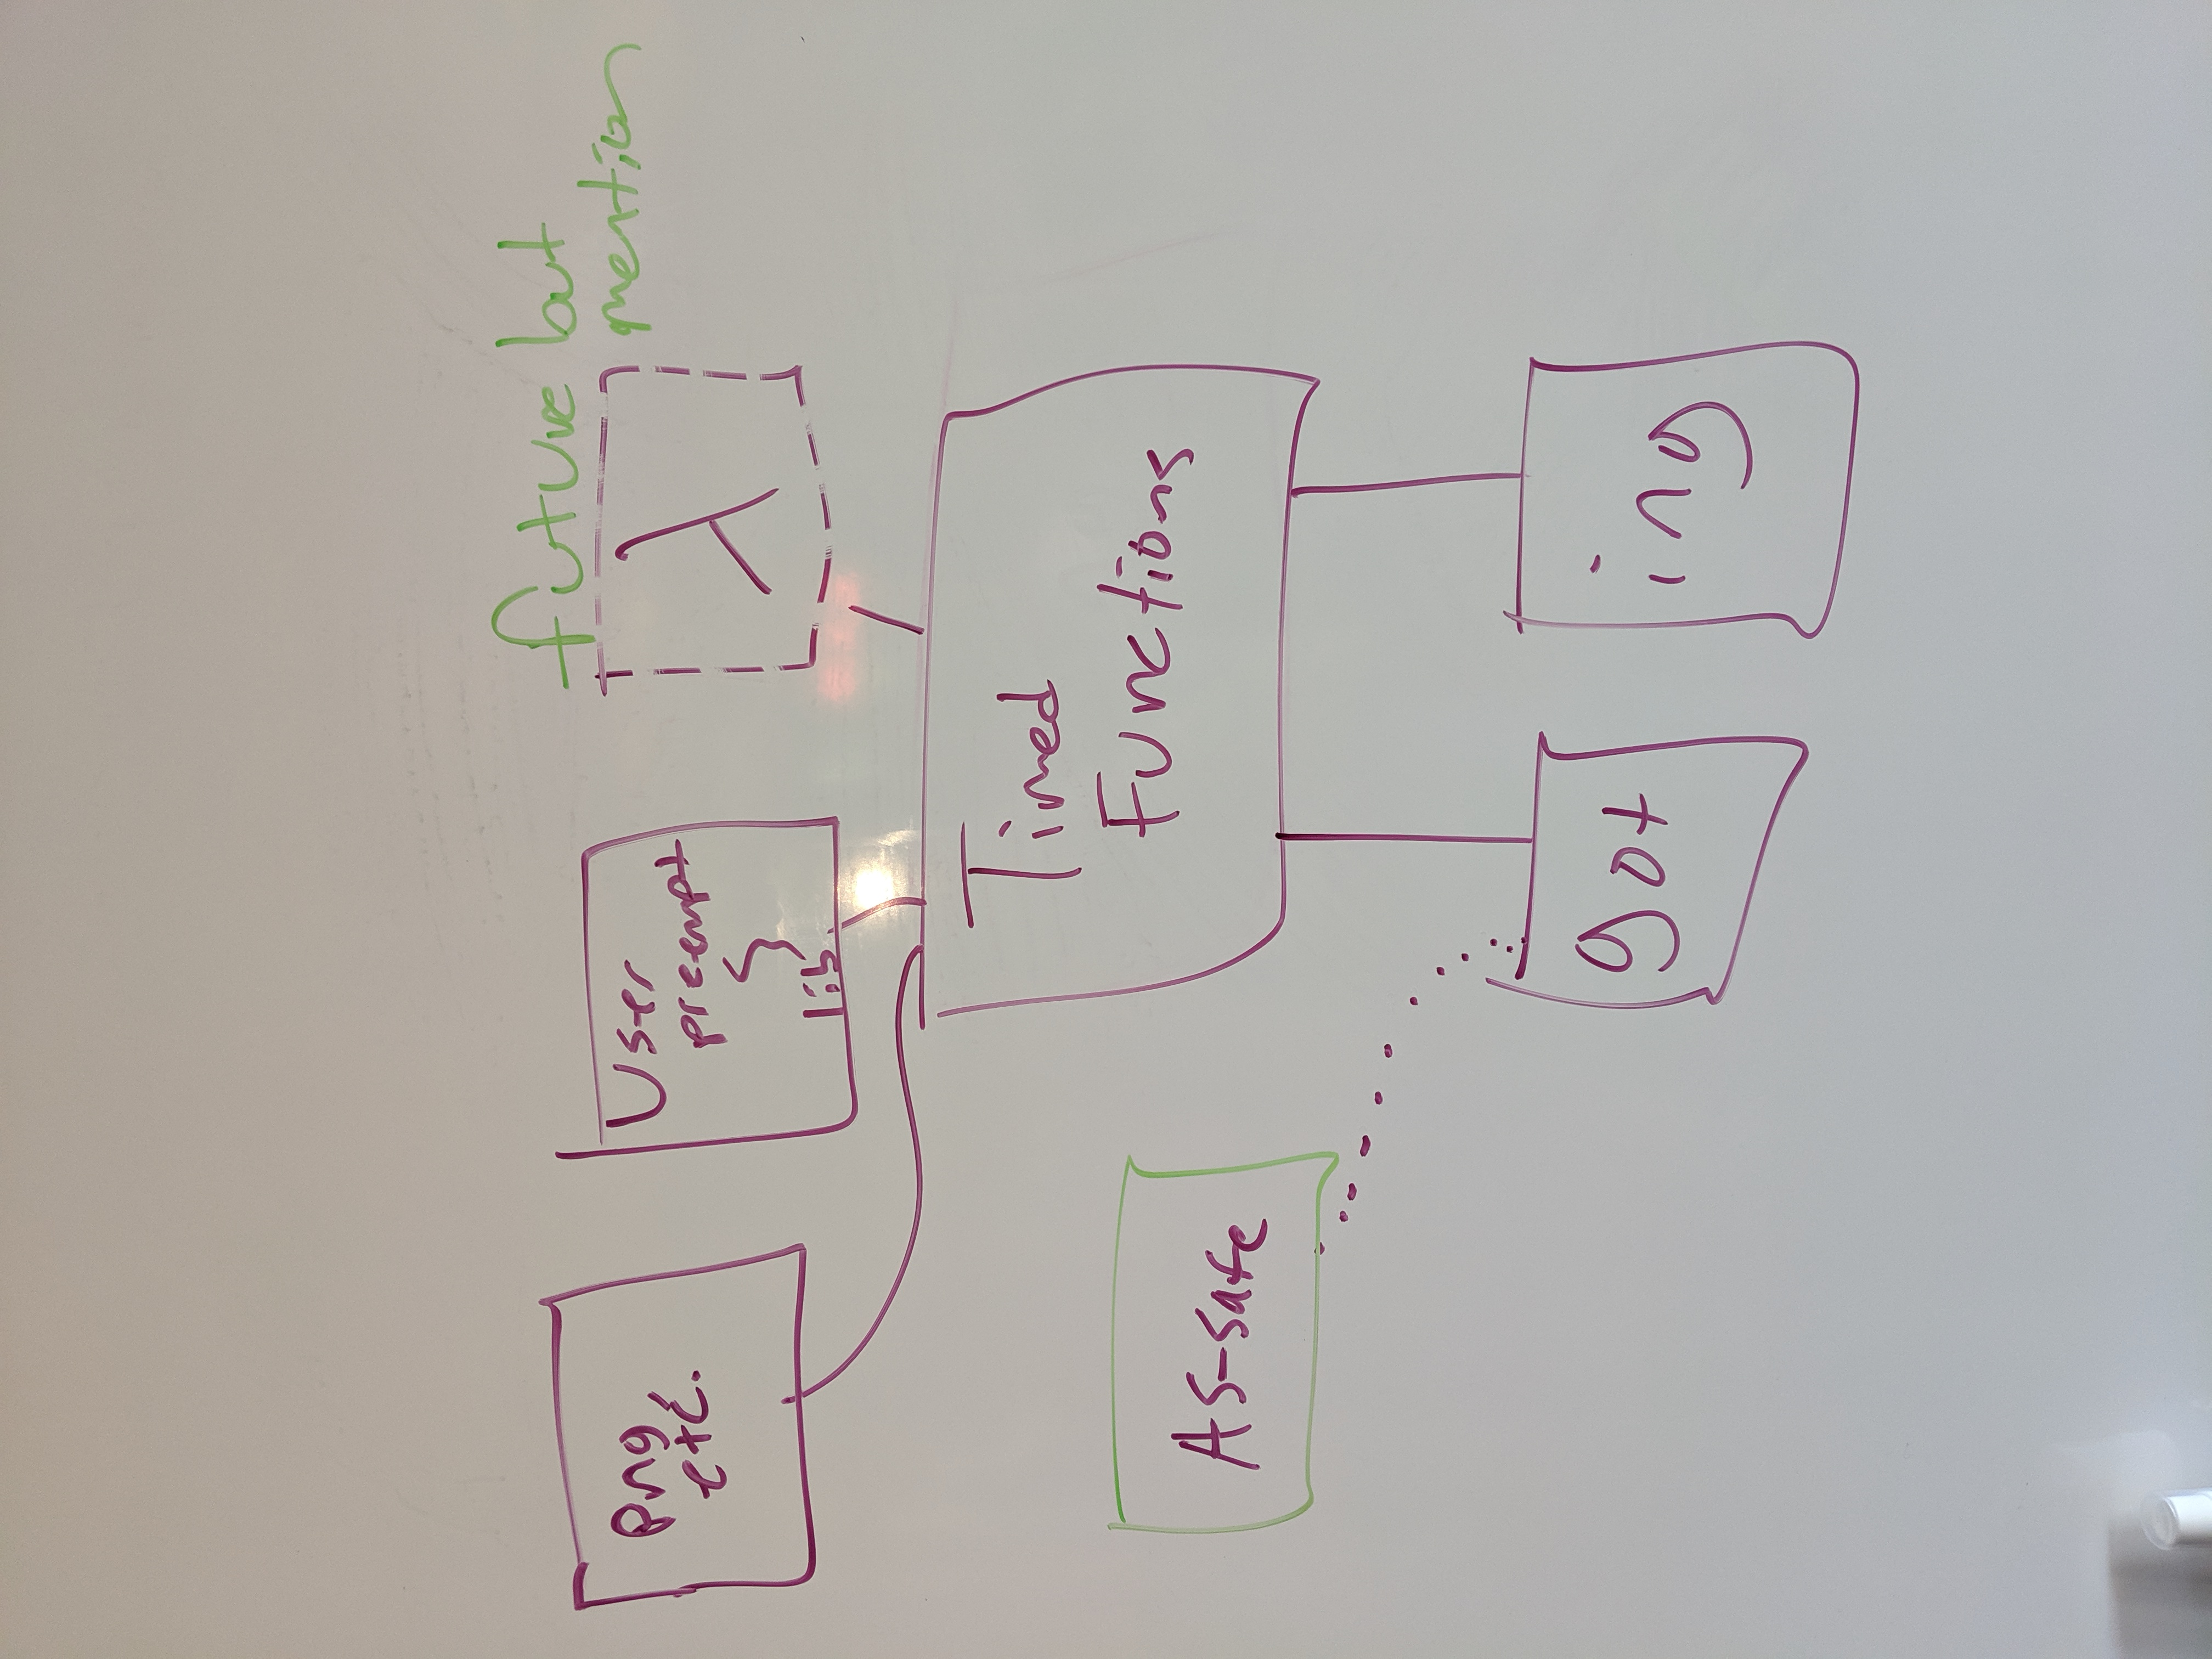
\includegraphics[width=0.75\columnwidth]{figs/architecture}
\end{center}
\caption{The preemptible functions software stack.  \textnormal{Rectangular boxes
represent components implementing the preemptible functions abstraction.  Ovals
represent components built on top of these.  Hexagonal boxes show the
required runtime environment.}}
\label{fig:architecture}
\end{figure}


\subsection{Automatic handling of shared state}

As we found in Section~\ref{sec:intro}, a key design challenge facing
\textit{libinger} is the shared state problem:  Suppose a preemptible function
$\mathcal{F}_0$ calls a stateful routine in a third-party library $\mathcal{L}$, and
that $\mathcal{F}_0$ times out and is preempted by \textit{libinger}.  Later, the
user invokes another timed function $\mathcal{F}_0'$, which also calls a stateful
routine in $\mathcal{L}$.  This constituting a concurrency violation,
\textit{libinger} must hide state modifications in $\mathcal{L}$ by $\mathcal{F}_0$
from the execution of $\mathcal{F}_0'$ to avoid undefined behavior.

The problem is actually even worse.  Those familiar with POSIX signals may notice
that, upon a function's timeout, its caller interrupts it.  \textit{The rest of the
program} can therefore be viewed as a signal handler, and would normally be expected
to restrict itself to calling async-signal-safe (roughly, nonreentrant)
functions~\cite{signal-safety-manpage}.

One non-solution to this problem is to instead prevent preemptible functions from
calling into third-party code (Section~\ref{sec:related}), because doing so would
severely limit their usefulness.  Instead, our approach
is to automatically and dynamically create copies of $\mathcal{L}$ to
isolate state from different timed functions. Doing so while running on
existing systems software (a requirement discussed next) requires solving many
design and implementation challenges, which we cover in our discussion of
\textit{libgotcha} in Section~\ref{sec:libgotcha}.


\subsection{Performance on unmodified system stacks}

Unlike prior work on low-latency preemptive scheduling such as
Shinjuku~\cite{Kaffes:nsdi2019}, \textit{libinger} runs on top of the existing
OS. An obvious design to achieve this goal would be to use a thread or process,
the existing concurrency mechanisms provided by the OS, but these mechanisms
are too slow. We choose a middle ground between the very fast but specialized
approaches like Shinjuku, and slow but fully-general OS approaches.


%\subsection{Language independence}
%
%Our interface is inspired by that of Scheme engines~\cite{haynes:iucs1984};
%however, since we seek language independence, there are some fundamental
%differences.  Most notably, our preemptible functions may contain
%state\footnote{In addition to lifting a restriction on timed code, this
%difference led us to make the \texttt{linger} type stateful as well, and allow
%the \texttt{resume()} function to mutate it in place rather than constructing a
%copy.  In another move to improve portability, we chose to make \texttt{linger}
%a structured type instead of a function, thereby avoiding dependence on
%languages supporting closures.  In languages with operator overloading, the
%preemptible function bindings may define a function-call operator that calls
%\texttt{resume()} to achieve Scheme-style surface syntax.}, something not
%handled by Scheme due to the functional nature of the language.  We simplify
%their API by returning the preemptible function's return value in the
%\texttt{linger} union rather than passing it to a success callback.  Our goal
%was to create a core API amenable to language-specific integration integration;
%for instance, in addition to the barebones C interface, our current
%implementation exposes a Rust interface that uses a first-class tagged union
%(sum type) to ensure at compile time that the caller has checked which variant
%a \texttt{linger} contains before using it.


\subsection{Execution stacks}

The \textit{libinger} library implements the preemptible function interface. Although
it provides users with the familiar function call interface, internally,
\textit{libinger} uses a combination of unstructured control flow in the form of
multiple stack regions and signal handlers. \textit{libinger} runs each timed
function on a separate stack, different from the user's own stack. This is
necessary to prevent different functions or the user from clobbering each
other's stack when some timed functions have been preempted.


\subsection{Timer interrupts}

\begin{figure}
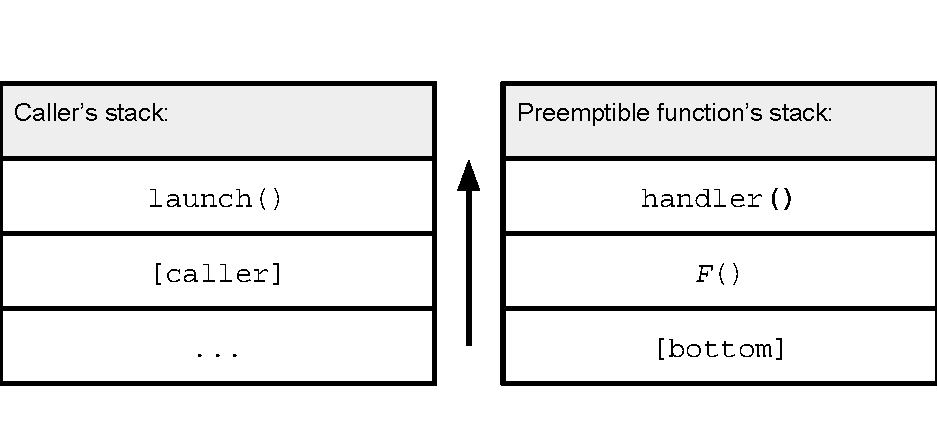
\includegraphics[width=\columnwidth]{figs/twostacks}
\caption{The stacks before and after a timeout.  \textnormal{Upon discovering
that the preemptible function has exceeded its time bound, the handler returns to the
checkpoint continuation within the \texttt{launch()} function, removing its own stack
frame in the process.  Then, \texttt{launch()} returns to the original call site,
which removes its stack frame.}}
\label{fig:twostacks}
\end{figure}

While \textit{libinger} is executing a executing the user-provided function, we
enable fine-grained timer interrupts to periodically run our signal handlers
that monitor the execution of the preemptible functions. While a preemptible
function is running, the timer interrupt fires periodically, causing the signal
handler to be invoked each time. If a function exceeds its timeout, \textit{libinger}
jumps back to the caller, returning a continuation that stores the preemptible
function's register values.

Figure~\ref{fig:twostacks} shows the two stacks of execution, belonging to the
\textit{libinger} user and the preemptible function, present while the signal handler
is running. It also shows what happens to the stack frames of both if the
function times out. The handler first checks whether the preemption signal was
intended for the current thread, as described earlier.  It then checks whether
the preemptible function has exceeded its timeout; if so, it swaps the contents
of the signal handler's continuation (accessible via the final argument to the
function~\cite{sigaction-manpage}) with the checkpoint continuation saved by
\texttt{launch()}.  This causes the subsequent return from the signal handler
to jump back to \texttt{launch()}, which then returns a \texttt{linger}
structure containing the signal handler's original context.  A subsequent
\texttt{resume()} call on this packaged continuation proceeds in much the same
way as \texttt{launch()}, but resumes the original computation by sending
itself a special signal with \texttt{pthread\_kill()}, then swapping the saved
context with the contents of that handler's context\footnote{This is necessary
because POSIX left the semantics of calling \texttt{setcontext()} on the
continuation saved by a signal handler invocation unspecified, leading
implementations such as GNU not to handle this
case~\cite{getcontext-manpage}.}.

When the caller is finished with a preemptible function, it must deallocate it
either explicitly (C) or implicitly via the \texttt{inger} type's destructor
(Rust).  This cleans up the \textit{libinger} resources allocated by
\texttt{launch()};
however, if the call constitutes a cancellation, the current implementation of
\textit{libinger} does not automatically clean up resources already allocated by the
preemptible function itself.  While the lack of a standard deinitialization API
makes this inherently hard to do in C, it is possible to implement in languages
such as Rust that support destructors.  For instance, the approach proposed by
Boucher et al.~\cite{boucher:atc2018} could be employed to raise a panic
(exception) on the preemptible function's stack, causing the language runtime
to unwind each stack frame, invoking the destructor of each local variable in
the process.


\subsection{Performance goals}

Although seeking to implement low-latency preemption without requiring a custom
operating system, we sought a design that could operate with performance
comparable to Shinjuku's.  Our prototype is not yet optimized to this extent,
but we provide a back of the envelope calculation of its minimum possible
preemption latency based on Shinjuku's comparison of the latency of bare-metal
interprocessor interrupts (IPIs) versus Linux signals (measured from their
request by one core to the invocation of the other's interrupt service routine
or signal handler).  While IPIs take an average of only 1993 cycles, compared
to 4950 for signals (a ratio of 1:2.5), a look at their sender/receiver
breakdown of the latter number suggests two opportunities to reduce this
overhead without abandoning the existing systems software stack:  First, 343 of
those cycles (6.9\%) are spent propagating the signal between the two cores,
and should largely disappear by initiating it on the same thread that is to be
preempted.  Second, 2084 cycles (42\%) are incurred by the sender, of which
some portion should also disappear~\cite{Kaffes:nsdi2019}.  We therefore expect
that an optimized system based on intra-thread signals built atop the existing
system stack could achieve an average preemption latency within 2.5x of that of
their custom operating system with a dedicated watchdog core.
